
\begin{abstract}
When does multi-task learning provide positive (or negative) information transfer, compared to single-task learning?
In this work, we address this question by studying
% the performance of predicting a particular task given multiple tasks.
a multi-task learning architecture that uses a shared layer for all tasks and a separate output layer for each task.
First, for the setting of high-dimensional linear regression, we show that the type of transfer is determined by the bias-variance tradeoff of multi-task learning estimators.
We provide a sharp analysis of the tradeoff and extend the result to transfer learning.
We develop a technical tool on the inverse of the sum of two random matrices that naturally arises from the analysis.
Second, we identify three components including task similarity, data size and covariate shift to explain negative transfer in multi-task learning rigorously.
Finally, we show practical implications of our theory for detecting and mitigating negative transfer.
We propose an incremental training scheduler for improving the efficiency of multi-task training for predicting a particular task.
We validate our theory and our proposed method on image and text classification tasks.
\end{abstract}

\section{Introduction}

%Multi-task learning is an inductive learning mechanism to improve generalization performance using related task data.
%Many state-of-the-art results in computer vision and natural language processing are obtained using multi-task learning.
Multi-task learning represents a powerful paradigm to solve complex tasks in computer vision \cite{chexnet17,ZSSGM18}, natural language processing \cite{GLUE,superglue} and many other areas \cite{ZY17}.
%In multi-task learning, having related task data is fundamental to its performance.
%Multi-task learning is particularly powerful when there is limited labeled data for a task to be solved, meanwhile more labeled data from different but related tasks is available.
By combining multiple information sources, it is possible to share all the information in the same model.
%For example, many applications in , and many other areas have been achieved by learning from multiple tasks together.
The performance of multi-task learning depends on the relationship of the information sources \cite{C97}.
When the information sources are heterogeneous, negative transfer--where multi-task learning (MTL)  performs worse than single-task learning (STL)--has often been observed \cite{PY09,AP16,BS17}.
While many empirical approaches have been proposed to mitigate negative transfer \cite{ZY17}, a precise understanding of when negative transfer occurs has remained elusive in the literature \cite{R17}.
%This phenomenon, known as \textit{negative transfer}, is fundamental to the understanding of multi-task learning.
In this work, we show that negative transfer is determined by the bias-variance tradeoff of multi-task learning estimators for the setting of high-dimensional linear regression. % for learning from multiple linear regression tasks.
We develop technical tools to analyze the tradeoff and use our tools to explain negative transfer precisely.
Inspired by the theory, we propose an incremental training schedule to improve multi-task training.
%We consider a setting where the target task has limited labeled data and show
%On the other hand, unless the structures across task data are well-understood, applying multi-task learning on several different datasets often result in suboptimal models (or negative transfer in more technical terms).

Identifying negative transfer requires developing tight generalization bounds for both multi-task learning and single-task learning.
In classical Rademacher or VC based theory of multi-task learning \cite{B00,AZ05,M06}, the generalization bounds are usually presented so that the error reduces as the data sizes of all tasks increase.
For instance, the data sizes of all tasks are often assumed to be equal \cite{B00}.
On the other hand, uneven data sizes or dominating tasks have been empirically observed as a cause of negative transfer \cite{YKGLHF20}.
More recent work has shown the benefit of learning multi-task representations for certain half-spaces \cite{MPR16} and sparse regression \cite{LPTV09,LPVT11}.
\todo{Add our ICLR work here.}
\squishlist
	\item \textbf{Task similarity:}
	\item \textbf{Data sizes:}
	\item \textbf{Covariate shift:}
\squishend
To rigorously study negative transfer, the technical challenge is to develop generalization bounds that scale tightly with properties of the data.


In this work, we consider the setting of high-dimensional linear regression and focus on predicting a particular task that only contains limited amount of labeled data.
Following Hastie et al. \cite{HMRT19} and Bartlett et al. \cite{BLLT20}, we assume that for every task $1\le i\le t$, its features are random vectors $x = \Sigma_i^{1/2}z$, where $z\in\real^p$ consists of i.i.d. entries with mean zero and unit variance, and $\Sigma_i\in\real^{p\times p}$ is a positive semidefinite matrix.
Let $n_i$ denote the data size and $X_i\in\real^{n_i\times p}$ denote the features of task $i$.
The labels of task $i$ are given by $Y_i = X_i\beta_i + \varepsilon_i$, where $\beta_i\in\real^p$ denotes task $i$'s ground truth parameters and $\varepsilon_i$ denotes i.i.d. random noise with mean zero and variance $\sigma^2$.
Without loss of generality, let the $t$-th task denote the target task.
Importantly, the target task's data size is a fixed constant times $p$ in the high-dimensional setting.
Hence adding more labeled data can help improve its test performance.
%We shall assume that each task data follows a linear model, i.e. $y_i = X_i \beta_i + \varepsilon_i$, $1\le i\le k$.
%Here $\beta_i\in\real^p$ is the model parameter for the $i$-th task.
%Each row of $X_i\in\real^{n_i\times p}$ is assumed to be drawn i.i.d. from a fixed
%distribution with covariance matrix $\Sigma_i$.
We focus on the hard parameter sharing architecture with a linear shared layer $B\in\real^{p\times r}$ for all tasks and a separate prediction head $\set{W_i \in \real^{r}}_{i=1}^t$ for each task \cite{R17,MTDNN19,WZR20}.
%This corresponds to minimizing $ \sum_{i=1}^t \norm{X_i B W_i - Y_i}^2$.
Let $\hat{\beta}_t^{\MTL} = B W_t$ denote the optimal multi-task estimator for the target task.
Let $\hat{\beta}_t^{\STL}$ denote the single-task estimator.
We define these precisely in Section \ref{sec_setup}.
We say there is negative transfer if the prediction loss of $\hat{\beta}_t^{\MTL}$  is larger than that of $\hat{\beta}_t^{\STL}$, or positive transfer otherwise.


\begin{figure}[!t]
	\begin{subfigure}[b]{0.32\textwidth}
		\centering
		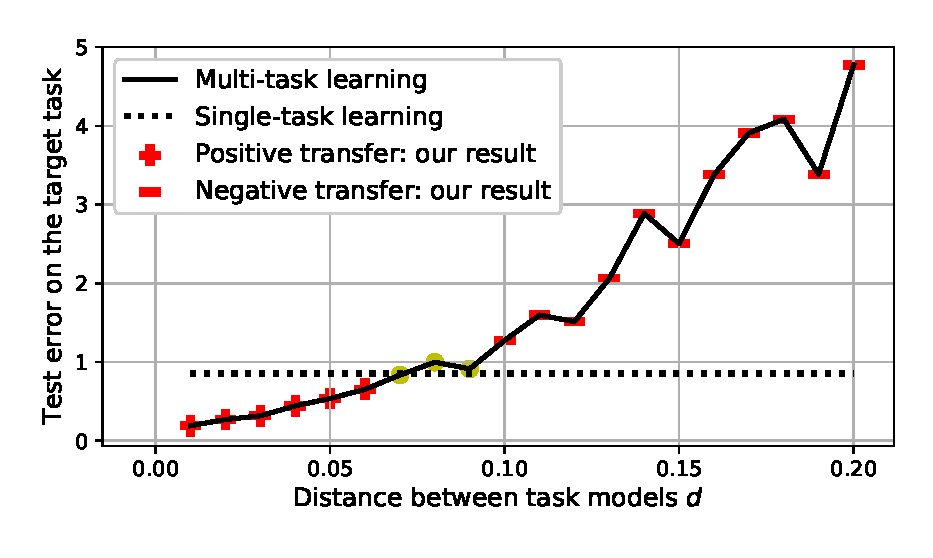
\includegraphics[width=0.98\textwidth]{figures/model_shift_phase_transition.eps}
		\caption{Task similarity}
		\label{fig_model_shift}
	\end{subfigure}\hfill
	\begin{subfigure}[b]{0.32\textwidth}
		\centering
		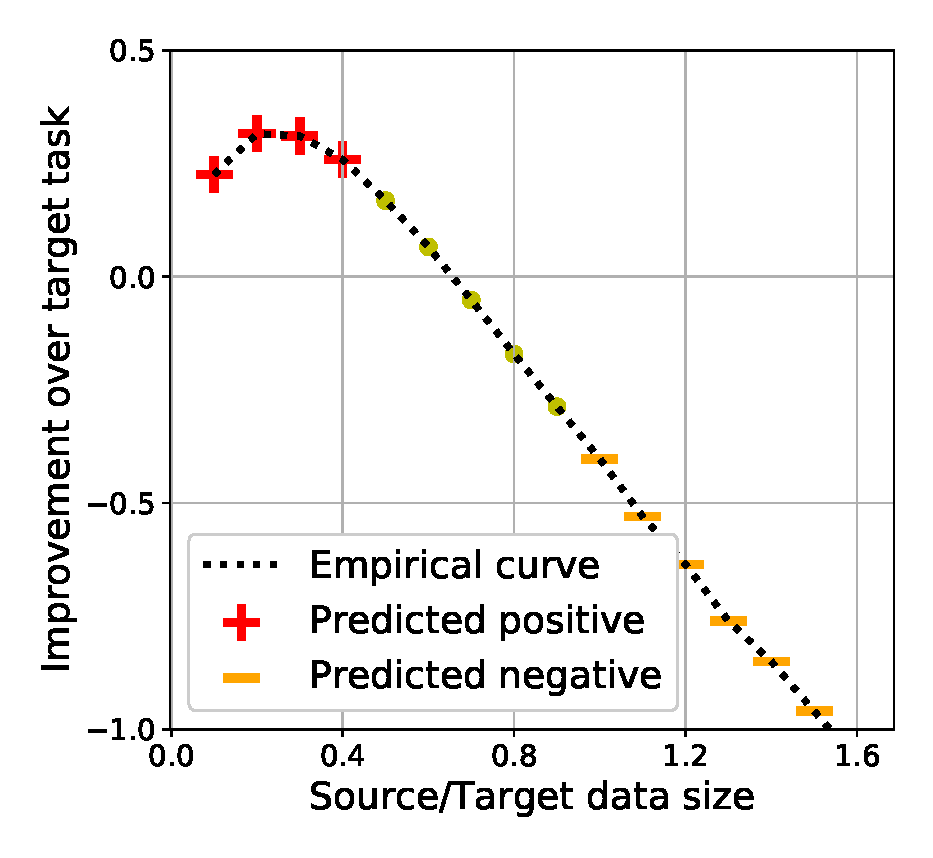
\includegraphics[width=0.98\textwidth]{figures/datapoints_phase_transition.eps}
		\caption{Data sizes}
		\label{fig_size}
	\end{subfigure}\hfill
	\begin{subfigure}[b]{0.32\textwidth}
		\centering
		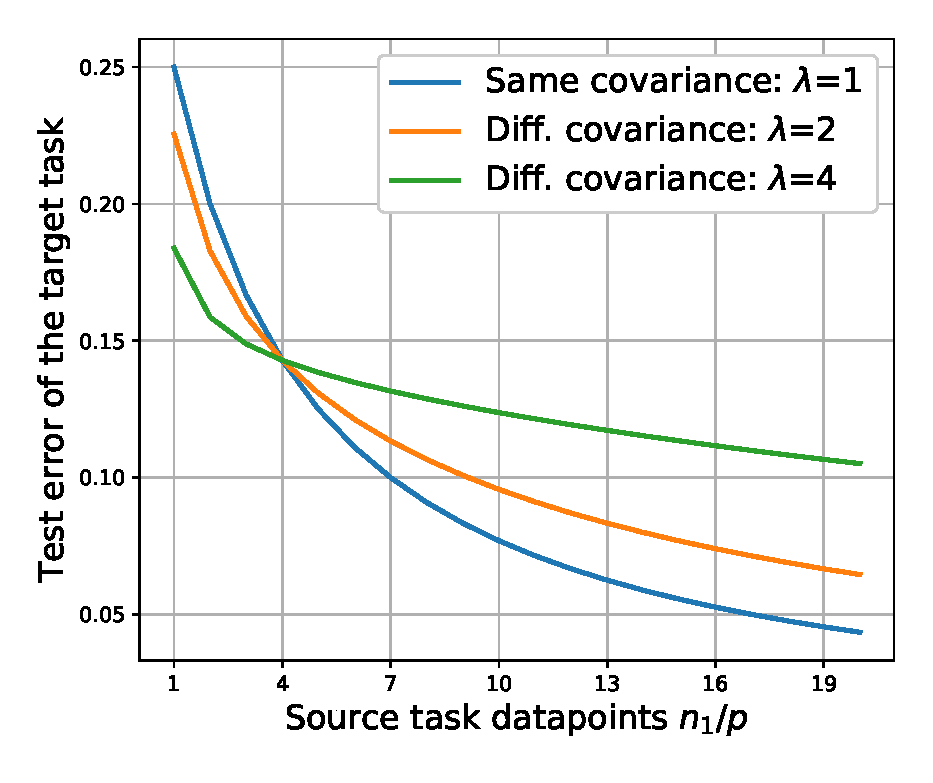
\includegraphics[width=0.98\textwidth]{figures/complementary.eps}
		\caption{Covariate shift}
		\label{fig_covariate}
	\end{subfigure}
	\caption{Three takeaways of our theory in Section \ref{sec_insight}.
	(a) As task model distance increases, we observe a transition from positive to negative transfer  (Proposition \ref{prop_dist_transition}).
	(b) As source/target data ratio increases, we observe a transition from positive to negative transfer (Proposition \ref{prop_data_size}).
	(c) As covariate shift gets more severe (measured by increasing $\lambda$), MTL performance gets worse (Proposition \ref{prop_covariate}).
	The $y$-axis measures the performance of MTL minus STL.}
	\label{fig_model_shift_phasetrans}
	\vspace{-0.2in}
\end{figure}

\textbf{Main results.}
We revisit the bias-variance tradeoff of the multi-task estimator.
Interestingly, we observe that the variance of the multi-task estimator is always smaller than the variance of the single-task estimator, hence resulting in a positive effect of variance reduction.
The bias of the multi-task estimator results in a negative effect caused by the difference between $\beta_t$ and the rest of $\set{\beta_i}_{i=1}^{t-1}$.
Hence, the bias-variance tradeoff determines whether we observe positive or negative transfer.

Our first contribution is to develop a new technical tool for a quantity that arises naturally from the analysis of two tasks.
Concretely, we show a tight bound on the trace of $(X_1^{\top}X_1 + X_2^{\top}X_2)^{-1}$, which extends a well-known result on the trace of $(X_1^{\top}X_1)^{-1}$ for the single-task setting \cite{S07}.
Our analysis yields nearly optimal concentration error, which may be of independent interest.
Using this tool, we show the following results in Section \ref{sec_main}.
\squishlist
	\item We provide a sharp analysis of the bias-variance tradeoff of $\hat{\beta}_t^{\MTL}$ for two settings:
(i) two tasks with general covariance matrice; (ii) any number of tasks that have the same features (e.g. images).
	\item We extend our result to transfer learning in the setting of high-dimensional linear regression.
	We pool learnt source task representations into a shared body similar to $B$ in the hard parameter sharing architecture, as in Taskonomy by Zamir et al. \cite{ZSSGM18}.
	We show that the model shift bias can be captured by the projection of $\beta_t$ to the orthogonal subspace spanned by $\set{\beta_i}_{i=1}^{t-1}$.
\squishend

Our second contribution is to use our newly developed tool to explain negative transfer in multi-task learning rigorously.
In Section \ref{sec_insight}, we consider three components including task similarity, data size and covariate shift for a simplified isotropic setting of two tasks.
We measure task similarity by how small is the distance between $\beta_1$ and $\beta_2$.
Using our tool, we explain a transition from positive to negative transfer as task similarity decreases.
%		Furthermore, we show that negative transfer is more likely to occur when the source task labels are particularly noisy.
%		In Section \ref{sec_validate}, we validate the observation on text and image classification tasks.
%	In , we provide the trade-off between $\norm{\beta_1 - \beta_2}^2$ and a certain function $\Phi(\rho_1, \rho_2)$ to determine the type of transfer.
We show that increasing the data size of the source task does not always improve performance for the target task in multi-task learning.
	Then, we analyze the benefit of multi-task learning for reducing the amount of labeled data needed to achieve comparable performance to single-task learning, which is a key empirical finding of Taskonomy.
We show that covariate shift, measured by $\Sigma_1^{1/2}\Sigma_2^{-1/2}$, is another cause for suboptimal performance for $\hat{\beta}_t^{\MTL}$.
		We show that as $n_1 / n_2$ becomes large, having no covariate shift between the source and target tasks yields the optimal performance for the target task.
%		On the other hand, when $n_1 / n_2$ is small, there are counter examples where having the same covariance matrix is not necessarily the optimal choice.

Our last contribution is to connect our theory to practical problems of interest.
(i) We provide a single-task based metric to predict positive or negative transfer in multi-task learning.
While it is not well understood when multi-task learning provides positive transfer, we show that the STL results can help indicate and understand MTL results on ChestX-ray14 \cite{chexnet17} and sentiment analysis datasets \cite{LZWDA18}.
(ii) We design an incremental training schedule to improve the efficiency of multi-task training for predicting a particular task.
We show that our training schedule reduces the computational cost by $55\%$ compared to baseline multi-task training on the sentiment analysis dataset, while keeping the accuracy the same.
(iii) We validate the three components of our theory in Section \ref{sec_insight} and measure the data efficiency of multi-task learning on the sentiment analysis dataset.

